\documentclass{article}
\usepackage{graphicx} % Required for inserting images
\usepackage{amsmath}
\usepackage[hidelinks]{hyperref}
\usepackage{subcaption}
\usepackage{tikz}
\usepackage{braket}
%\usepackage{minted}
\usepackage{pseudo}
\usepackage{mathtools}
\usepackage{tabto}
\usepackage{float}
\usepackage{titlesec}
\usetikzlibrary{shapes.geometric}
\usetikzlibrary{calc}
\title{Efficient Classical Simulation of the Quantum Fourier Transform}
\author{
\centering
\begin{tabular}{r|c|l}
    & Asmus Tørsleff & asmt@itu.dk (asmus.torsleff@gmail.com)\\
    Supervisor & Michael Kastoryano & micka@itu.dk \\
    Co-Supervisor & Nutan Limaye & nuli@itu.dk \\
\end{tabular}}
\date{\today}
\TabPositions{1.5cm} % Adjust as needed!
\setcounter{MaxMatrixCols}{20}
\begin{document}

\maketitle
\begin{center}
    code: BIBAPRO1PE
\end{center}
\newpage
\tableofcontents
\newpage
\section{Motivation}
%\newpage
%\input{introduction}
\newpage
\section{Dense Simulation}\label{sec:dense}
We want to simulate applying the QFT to some state, for this we need a way to represent the QFT and the state. 
In this section we will work towards representing the QFT circuit as a matrix and the state as a vector. 
\subsection{Representing a one qubit state}
In classical computation a bit can either be 1 or 0, in quantum systems however a qubit has a certain probability of collapsing to either one or zero at a given time.
To simulate this we use a vector to represent a qubit or a system of qubits, we denote this using Dirac notation. In Dirac notation we have a bra $\bra{}$ and a ket $\ket{}$, generally a bra denotes a row vector and a ket denotes a column vector.
To extract the probabilities of a qubit or system of qubits collapsing to one state or the other we take the norm squared of the entries in the vector, the sum of these must be 1 to be a valid state.
\newcommand{\qo}{\begin{bmatrix}
        0\\
        1\\
    \end{bmatrix}}
\newcommand{\qz}{\begin{bmatrix}
        1\\
        0\\
    \end{bmatrix}}
\newcommand{\qp}{\begin{bmatrix}
        \sqrt{0.5}\\
        \sqrt{0.5}\\
    \end{bmatrix}}
\newcommand{\qm}{\begin{bmatrix}
        \sqrt{0.5}\\
        -\sqrt{0.5}\\
    \end{bmatrix}}
    
\newcommand{\qto}{\mathbf{1}}
\newcommand{\qtz}{\mathbf{0}}
\newcommand{\qtp}{\textbf{+}}
\newcommand{\qtm}{\textbf{--}}
\newcommand{\qti}{\mathbf{I}}
\newcommand{\qtr}[1]{\mathbf{R_{#1}}}
\newcommand{\qtx}{\mathbf{X}}
\newcommand{\qth}{\mathbf{H}}
\newcommand{\qtcx}{\mathbf{CX}}
\begin{figure}[H]
    \centering
    \begin{equation*}
        \ket{\qto} =\qo    
    \end{equation*}
    \caption{A qubit with a probability of 1 of collapsing 
    to one}
    \label{fig:q1}
\end{figure}
\begin{figure}[H]
    \centering
    \begin{equation*}
        \ket{\qtz} =\qz
    \end{equation*}
    \caption{A qubit with a probability of 1 of collapsing to zero}
    \label{fig:q0}
\end{figure}
\begin{figure}[H]
    \centering
    \begin{align*}
    \ket{\qtp} &= \sqrt{0.5}(\ket{\qtz} + \ket{\qto}) = \qp\\
    \ket{\qtm} &= \sqrt{0.5}(\ket{\qtz} - \ket{\qto}) = \qm
    \end{align*}
    \caption{Qubits with a probability of 0.5 of collapsing to zero and one}
    \label{fig:q+}
\end{figure}
\noindent
In general a qubit
$
\begin{bmatrix}
    \alpha\\
    \beta\\
\end{bmatrix}
= \alpha \ket{\qtz} + \beta \ket{\qto}
$
has a probability of $|\alpha|^2$ of collapsing to zero and $|\beta|^2$ of collapsing to one.
Since we use a vector of complex numbers $|x|^2=xx^*$ denotes the norm squared, where if $x=a+bi$ then $x^*$ is the complex conjugate of $x$, $x^* =a-bi$.
For readabilitys sake we will not write $+bi$ after a number if $b=0$, you can assume all numbers in vectors and matricies are complex.

\vspace{\baselineskip}
\noindent
If we look at these vectors in a coordinate system, where the z axis is the imaginary axis, they all lie on a unit circle.
\begin{figure}[H]
    \centering
    \begin{tikzpicture}
        \draw[] (0,0) circle (3);
        
        \draw[->, thin] (0,-4) -- (0,4) node[draw=none,fill=none,font=\scriptsize,left]{y};
        \draw[->, thin] (-4,0) -- (4,0) node[draw=none,fill=none,font=\scriptsize,below]{x};
        
        \draw[thin](0.6, 3) -- (-0.6, 3) node[draw=none,fill=none,font=\scriptsize,left]{1};
        \draw[thin](3,0.6) -- (3,-0.6) node[draw=none,fill=none,font=\scriptsize,below]{1};
        
        \draw[->, thick] (0,0) -- (0,3) node[draw=none,fill=none,font=\scriptsize,midway,left]{$\ket{\qto}$};
        \draw[->, thick] (0,0) -- (3,0) node[draw=none,fill=none,font=\scriptsize,midway,above]{$\ket{\qtz}$};
        \draw[->, thick] (0,0) -- (2.1,2.1) node[draw=none,fill=none,font=\scriptsize,midway,left]{$\ket{\qtp}$};
        \draw[->, thick] (0,0) -- (2.1,-2.1) node[draw=none,fill=none,font=\scriptsize,midway,above]{$\ket{\qtm}$};
    \end{tikzpicture}
    \caption{'Bloch circle' with vectors $\ket{\qto}$, $\ket{\qtp}$, $\ket{\qtz}$ and $\ket{\qtm}$ plotted}
    \label{fig:block_cirkle}
\end{figure}

\noindent
In reality we often use complex numbers with a non-zero imaginary part in the vectors, which results in the qubit states instead lying on the unit sphere, this is known as the Bloch sphere. The z axis is called the phase and generally has no impact on the probabilities of collapsing to a certain state, however it can be used to hold extra information before the qubit is collapsed, this can be useful in computations.

\subsection{Multiple qubit states}
$\ket{\qto\qtp\qtm}$ denotes a system collapsing to either $\ket{\qto\qtz\qtz}$, $\ket{\qto\qtz\qto}$, $\ket{\qto\qto\qtz}$ or $\ket{\qto\qto\qto}$ with probability 0.25. 
If we want to compute the state vector for the whole system we take the Kronecker product\cite{kronecker_product}, sometimes called the tensor product, of the vectors representing the individual qubits in the system. 
The Kronecker product of two matrix like objects consists of duplicating the second object for every entry in the first object and then scaling every value in the duplicate by the entry in the first object.
\begin{figure}[H]
    \centering
    \begin{gather*}
        \begin{bmatrix}
            a_{00} & a_{01} & a_{02} \\
            a_{10} & a_{11} & a_{12} \\
        \end{bmatrix}
        \otimes
        \begin{bmatrix}
            b_{00} & b_{01} \\
            b_{10} & b_{11} \\
            b_{20} & b_{21} \\
        \end{bmatrix}
        = \\
        \begin{bmatrix}
            a_{00}
            \begin{bmatrix}
                b_{00} & b_{01} \\
                b_{10} & b_{11} \\
                b_{20} & b_{21} \\
            \end{bmatrix} 
            & a_{01}
            \begin{bmatrix}
                b_{00} & b_{01} \\
                b_{10} & b_{11} \\
                b_{20} & b_{21} \\
            \end{bmatrix} 
            & a_{02}
            \begin{bmatrix}
                b_{00} & b_{01} \\
                b_{10} & b_{11} \\
                b_{20} & b_{21} \\
            \end{bmatrix} \\
            a_{10}
            \begin{bmatrix}
                b_{00} & b_{01} \\
                b_{10} & b_{11} \\
                b_{20} & b_{21} \\
            \end{bmatrix} 
            & a_{11}\begin{bmatrix}
                b_{00} & b_{01} \\
                b_{10} & b_{11} \\
                b_{20} & b_{21} \\
            \end{bmatrix} 
            & a_{12}\begin{bmatrix}
                b_{00} & b_{01} \\
                b_{10} & b_{11} \\
                b_{20} & b_{21} \\
            \end{bmatrix} \\
        \end{bmatrix}
        =\\
        \begin{bmatrix}
            a_{00}b_{00} & a_{00}b_{01} & a_{01}b_{00} & a_{01}b_{01} & a_{02}b_{00} & a_{02}b_{01}\\
            a_{00}b_{10} & a_{00}b_{11} & a_{01}b_{10} & a_{01}b_{11} & a_{02}b_{10} & a_{02}b_{11}\\
            a_{00}b_{20} & a_{00}b_{21} & a_{01}b_{20} & a_{01}b_{21} & a_{02}b_{20} & a_{02}b_{21}\\
            a_{10}b_{00} & a_{10}b_{01} & a_{11}b_{00} & a_{11}b_{01} & a_{12}b_{00} & a_{12}b_{01}\\
            a_{10}b_{10} & a_{10}b_{11} & a_{11}b_{10} & a_{11}b_{11} & a_{12}b_{10} & a_{12}b_{11}\\
            a_{10}b_{20} & a_{10}b_{21} & a_{11}b_{20} & a_{11}b_{21} & a_{12}b_{20} & a_{12}b_{21}\\
        \end{bmatrix}
    \end{gather*}    
    \caption{Example of taking the Kronecker product of two matricies}
    \label{fig:Kronecker_example}
\end{figure}

\begin{figure}[H]
    \centering
    \begin{gather*}
        \ket{\qto\qtp\qtm} = \ket{\qto}\otimes\ket{\qtp}\otimes\ket{\qtm} = \\
        \qo\otimes\qp\otimes\qm = \\
        \begin{bmatrix}
            0
            \begin{bmatrix}
                \sqrt{0.5}
                \begin{bmatrix}
                    \sqrt{0.5}\\
                    -\sqrt{0.5}\\
                \end{bmatrix}\\
                \sqrt{0.5}
                \begin{bmatrix}
                    \sqrt{0.5}\\
                    -\sqrt{0.5}\\
                \end{bmatrix}\\
            \end{bmatrix}\\
            1
            \begin{bmatrix}
                \sqrt{0.5}
                \begin{bmatrix}
                    \sqrt{0.5}\\
                    -\sqrt{0.5}\\
                \end{bmatrix}\\
                \sqrt{0.5}
                \begin{bmatrix}
                    \sqrt{0.5}\\
                    -\sqrt{0.5}\\
                \end{bmatrix}\\
            \end{bmatrix}\\
        \end{bmatrix}= 
        \begin{bmatrix}
            0
            \begin{bmatrix}
                0.5\\
                -0.5\\
                0.5\\
                -0.5\\
            \end{bmatrix}\\
            1
            \begin{bmatrix}
                0.5\\
                -0.5\\
                0.5\\
                -0.5\\
            \end{bmatrix}\\
        \end{bmatrix}= 
        \begin{bmatrix}
            0\\
            0\\
            0\\
            0\\
            0.5\\
            -0.5\\
            0.5\\
            -0.5\\
        \end{bmatrix}
        =\\
        0\cdot\ket{\mathbf{000}} + 0\cdot\ket{\mathbf{001}}+ 0\cdot\ket{\mathbf{010}}+ 0\cdot\ket{\mathbf{011}}+\\
        0.5\cdot\ket{\mathbf{100}}- 0.5\cdot\ket{\mathbf{101}}+ 0.5\cdot\ket{\mathbf{110}}- 0.5\cdot\ket{\mathbf{111}}
    \end{gather*}
    \caption{Using the Kronecker product to compute the state vector for the system in state $\ket{\qto\qtp\qtm}$}
    \label{fig:multi_qubit_state_computation}
\end{figure}
\noindent
If we square this vector, equvilent to takeing the norm squared when the imaginary parts are zero,  we get the probability corresponding to each state.
\begin{figure}[H]
    \centering
    \begin{gather*}
        |\ket{\qto\qtp\qtm}|^2=
        \begin{bmatrix}
            0^2\\
            0^2\\
            0^2\\
            0^2\\
            0.5^2\\
            -0.5^2\\
            0.5^2\\
            -0.5^2\\
        \end{bmatrix}
        =
        \begin{bmatrix}
            0\\
            0\\
            0\\
            0\\
            0.25\\
            0.25\\
            0.25\\
            0.25\\
        \end{bmatrix}
    \end{gather*}
    \caption{Squaring entries the in state vector to obtain probabilities of the system being in each state, the $i$'th entry in the vector is the probability of the system being in state $\ket{i}$ if you write $i$ in binary using 3 digits}
    \label{fig:square_state}
\end{figure}

\subsection{Manipulating qubits}\label{sec:maniq}
\noindent
In traditional electrical circuits we use logic gates such as NOT, AND, OR, NAND, etc. to manipulate bits. In quantum circuits some common gates are Pauli-X (X, bit flip or NOT), I (identity), H (Hadamard), CNOT (CX or controlled not), etc. In the same way we represent the state of a quantum system as a vector, we can represent a gate that operates on a state as a matrix. 
\newcommand{\qi}{\begin{bmatrix}
        1 & 0\\
        0 & 1\\
    \end{bmatrix}}
\newcommand{\qre}[1]{\mathrm{e}^{\frac{2\pi \mathrm{i}}{2^{#1}}}}
\newcommand{\qr}[1]{\begin{bmatrix}
        1 & 0\\
        0 & \qre{#1}\\
    \end{bmatrix}}
\newcommand{\qx}{\begin{bmatrix}
        0 & 1\\
        1 & 0\\
    \end{bmatrix}}
\newcommand{\qh}{\begin{bmatrix}
        \sqrt{0.5} & \sqrt{0.5}\\
        \sqrt{0.5} & -\sqrt{0.5}\\
    \end{bmatrix}}
\newcommand{\qcx}{\begin{bmatrix}
        1 & 0 & 0 & 0\\
        0 & 1 & 0 & 0\\
        0 & 0 & 0 & 1\\
        0 & 0 & 1 & 0\\
    \end{bmatrix}}
    

\begin{figure}[H]
    \centering
    \begin{align*}
        \qti = \qi\quad
        \qtx = \qx\quad
        \qth = \qh\quad
        \qtr{n} = \qr{n}
    \end{align*}
    \caption{Matrixes corresponding to $\qti$, $\qtx$, $\qth$ and $\qtr{n}$ gates, which act on a single cubit}
    \label{fig:single_qubit_gates}
\end{figure}

\noindent
If we wish to apply a gate to a qubit in a system we do so by doing matrix multiplication between the state and the gate. 
\begin{figure}[H]
    \centering
    \begin{align*}
        \qti\ket{\qtz}=\ket{\qtz}\quad
        \qti\ket{\qto}=\ket{\qto}
    \end{align*}
    \caption{Applying $\qti$ gate to the states $\ket{\qtz}$ and $\ket{\qto}$}
    \label{fig:i}
\end{figure}

\begin{figure}[H]
    \centering
    \begin{align*}
        \qtx\ket{\qtz}=\ket{\qto}\quad
        \qtx\ket{\qto}=\ket{\qtz}
    \end{align*}
    \caption{Applying $\qtx$ gate to the states $\ket{\qtz}$ and $\ket{\qto}$}
    \label{fig:x}
\end{figure}

\begin{figure}[H]
    \centering
    \begin{align*}
        \qth\ket{\qtz}=\ket{\qtp}\quad
        \qth\ket{\qto}=\ket{\qtm}
    \end{align*}
    \caption{Applying $\qth$ gate to the states $\ket{\qtz}$ and $\ket{\qto}$}
    \label{fig:h}
\end{figure}

\begin{figure}[H]
    \centering
    \begin{align*}
        \qtr{2}\ket{\qtz}=\ket{\qtz}\quad
        \qtr{2}\ket{\qto}=
        \begin{bmatrix}
            0\\
            \mathrm{i}\\
        \end{bmatrix}
    \end{align*}
    \caption{Applying $\qtr{2}$ gate to the states $\ket{\qtz}$ and $\ket{\qto}$}
    \label{fig:r2}
\end{figure}

\begin{figure}[H]
    \centering
    \begin{align*}
        \qtcx\ket{\qtz\qtz}=\ket{\qtz\qtz}\quad
        \qtcx\ket{\qtz\qto}=\ket{\qtz\qto}\quad
        \qtcx\ket{\qto\qtz}=\ket{\qto\qto}\quad
        \qtcx\ket{\qto\qto}=\ket{\qto\qtz}
    \end{align*}
    \caption{Applying $\qtcx$ gate to the states $\ket{\qtz\qtz}$, $\ket{\qtz\qto}$, $\ket{\qto\qtz}$ and $\ket{\qto\qto}$}
    \label{fig:cx}
\end{figure}
\noindent
See appendix \ref{app:maniq} for detailed calculations of these applications. 

\vspace{\baselineskip}
\noindent
Here we see that applying $\qti$ does not change the state. Applying $\qtx$ takes the state to the same state but reversed. Applying $\qth$ takes the state into a super position of $\ket{\qto}$ and $\ket{\qtz}$. Applying $\qtr{n}$ changes the phase of the cubit but not the chance of it collapsing to something. 
A key property of quantum gates is that they are reversible, and in fact their own inverses. 
\begin{figure}[H]
    \centering
    \begin{align*}
        \qti(\qti\ket{\qtz})=\ket{\qtz}\quad
        \qti(\qti\ket{\qto})=\ket{\qto}
    \end{align*}
    \caption{Applying $\qti$ gate to the states $\ket{\qtz}$ and $\ket{\qto}$ twice}
    \label{fig:i2}
\end{figure}

\begin{figure}[H]
    \centering
    \begin{align*}
        \qtx(\qtx\ket{\qtz})=\ket{\qtz}\quad
        \qtx(\qtx\ket{\qto})=\ket{\qto}
    \end{align*}
    \caption{Applying $\qtx$ gate to the states $\ket{\qtz}$ and $\ket{\qto}$ twice}
    \label{fig:x2}
\end{figure}

\begin{figure}[H]
    \centering
    \begin{align*}
        \qth(\qth\ket{\qtz})=\ket{\qtz}\quad
        \qth(\qth\ket{\qto})=\ket{\qto}
    \end{align*}
    \caption{Applying $\qth$ gate to the states $\ket{\qtz}$ and $\ket{\qto}$ twice}
    \label{fig:h2}
\end{figure}

\begin{figure}[H]
    \centering
    \begin{align*}
        \qtr{2}(\qtr{2}\ket{\qtz})=\ket{\qtz}\quad
        \qtr{2}(\qtr{2}\ket{\qto})=\ket{\qto}
    \end{align*}
    \caption{Applying $\qtr{2}$ gate to the states $\ket{\qtz}$ and $\ket{\qto}$ twice}
    \label{fig:r22}
\end{figure}

\begin{figure}[H]
    \centering
    \begin{align*}
        \qtcx(\qtcx\ket{\qtz\qtz})=\ket{\qtz\qtz} \quad        
        \qtcx(\qtcx\ket{\qtz\qto})=\ket{\qtz\qto} \quad
        \qtcx(\qtcx\ket{\qto\qtz})=\ket{\qto\qtz}\quad
        \qtcx(\qtcx\ket{\qto\qto})=\ket{\qto\qto}
    \end{align*}
    \caption{Applying $\qtcx$ gate to the states $\ket{\qtz\qtz}$, $\ket{\qtz\qto}$, $\ket{\qto\qtz}$ and $\ket{\qto\qto}$ twice}
    \label{fig:cx2}
\end{figure}
\noindent
This makes any quantum circuit constructed using these gates reversible.

\subsection{Manipulating qubits individually}\label{sec:maniqi}
We have seen how we apply a gate to a system of qubits the same size as the gate. 
If we want to apply a gate to the $i$'th qubit we construct a gate the same size as the system 
which acts with identity on every other qubit. We again use the Kronecker product for this. 

\begin{figure}[H]
    \centering
    \begin{align*}
        \left(\qti\otimes\qti\otimes\qtx\right)\ket{\qtz\qtz\qtz}=\ket{\qtz\qtz\qto}
    \end{align*}
    \caption{Applying $\qtx$ to the first qubit in a 3 qubit system}
    \label{fig:individual_application1}
\end{figure}


\begin{figure}[H]
    \centering
    \begin{align*}
        \left(\qti\otimes\qtx\otimes\qti\right)\ket{\qtz\qtz\qtz}=\ket{\qtz\qto\qtz}
    \end{align*}
    \caption{Applying $\qtx$ to the second qubit in a 3 qubit system}
    \label{fig:individual_application2}
\end{figure}
\begin{figure}[H]
    \centering
    \begin{align*}
        \left(\qtx\otimes\qti\otimes\qti\right)\ket{\qtz\qtz\qtz}=\ket{\qto\qtz\qtz}
    \end{align*}
    \caption{Applying $\qtx$ to the thrid qubit in a 3 qubit system}
    \label{fig:individual_application3}
\end{figure}
\noindent
If we want to apply multiple gates at a time we just replace the corresponding $\qti$ gates. 
\begin{figure}[H]
    \centering
    \begin{align*}
        \left(\qtx\otimes\qti\otimes\qth\right)\ket{\qtz\qtz\qtz}=\ket{\qto\qtz\qtp}
    \end{align*}
    \caption{Applying $\qtx$ to the thrid qubit and $\qth$ to the first qubit in a 3 qubit system}
    \label{fig:applying_multiple_gates}
\end{figure}
\noindent
See calculations in appendix \ref{app:maniqi}.

\vspace{\baselineskip}
\noindent
In general we can construct and apply any number of gates, $U_0,U_1,..,U_n$, to a state $\ket{\Psi}$ in sequence, this is in essence our quantum circuit. 
And because of the assosiative nature of matrix multiplication we can combine the entire circuit before applying it to different states! 
This saves tremendous amounts of resources when doing repetitative computations.
\begin{figure}[H]
    \centering
    \begin{gather*}
        U_0 U_1 .. U_n \ket{\Psi} = \left(\prod_{i=0}^n U_i\right) \ket{\Psi}\\
    \end{gather*}
    \caption{Associative nature of matrix multiplication}
    \label{fig:assosiative}
\end{figure}

\begin{figure}[H]
    \centering
    \begin{align*}
        \mathbf{U}=\qtcx  \left(\qti\otimes\qth\right) \left(\qti\otimes\qtx\right)        =
        \begin{bmatrix}
            \sqrt{0.5}  &  \sqrt{0.5} & 0 & 0 \\
            -\sqrt{0.5} &  \sqrt{0.5} & 0 & 0 \\
            0 & 0 & -\sqrt{0.5} & \sqrt{0.5} \\
            0 & 0 & \sqrt{0.5}  & \sqrt{0.5} \\
        \end{bmatrix}
    \end{align*}
    \caption{Computing a matrix representation of a circuit,$\mathbf{U}$, that first applies $\qtx$ then $\qth$ to the first qubit then $\qtcx$ to the first and second qubit}
    \label{fig:circuit_matrix}
\end{figure}
\begin{figure}[H]
    \begin{align*}
        \mathbf{U}\ket{\qtz\qtz}&=\ket{\qtz\qtm}\\
        \mathbf{U}\ket{\qtz\qto}&=\ket{\qtz\qtp}\\
        \mathbf{U}\ket{\qto\qtz}&=-\ket{\qto\qtm}\\
        \mathbf{U}\ket{\qto\qto}&=\ket{\qto\qtp}
    \end{align*}
    \caption{Applying the circuit represented by the matrix $\mathbf{U}$ from figure \ref{fig:circuit_matrix} to different states}
    \label{fig:applying_circuit}
\end{figure}


\subsection{Controlled gates}
\newcommand{\qtcr}[1]{\mathbf{CR_{#1}}}
We have described the $\qtr{n}$ gate but for the $QFT$ circuit we need it controlled by another qubit. We can construct a controlled gate out of any other gate, we simply take the gate that should happen if the control qubit is $\ket{\qtz}$ and place it in the top left qudrant of a matrix, then place what should happen if it is $\ket{\qto}$ in the bottom right qudrant. 
This can be expressed like so: 
\begin{figure}[H]
    \begin{align*}
        \mathbf{CU_{1,2}}=\ket{\qtz}\bra{\qtz}\otimes\qti + \ket{\qto}\bra{\qto}\otimes\mathbf{U}&=\\
        \begin{bmatrix}
            1 \\
            0 \\
        \end{bmatrix}
        \begin{bmatrix}
            1 & 0 \\
        \end{bmatrix}
        \otimes\qti + 
        \begin{bmatrix}
            0 \\
            1 \\
        \end{bmatrix}
        \begin{bmatrix}
            0 & 1 \\
        \end{bmatrix}
        \otimes\mathbf{U}&=\\
        \begin{bmatrix}
            1 & 0 \\
            0 & 0 \\
        \end{bmatrix}
        \otimes\qti + 
        \begin{bmatrix}
            0 & 0 \\
            0 & 1 \\
        \end{bmatrix}
        \otimes\mathbf{U}& 
    \end{align*}
    \caption{Constructing a controled gate $\mathbf{CU_{1,2}}$ from a gate $\mathbf{U}$ where the first cubit controlls the second}
    \label{fig:CU1}
\end{figure}
\begin{figure}[H]
    \begin{align*}
        \mathbf{CU_{2,1}}=\qti\otimes\ket{\qtz}\bra{\qtz} + \mathbf{U}\otimes\ket{\qto}\bra{\qto}&=\\
        \qti\otimes
        \begin{bmatrix}
            1 \\
            0 \\
        \end{bmatrix}
        \begin{bmatrix}
            1 & 0 \\
        \end{bmatrix}+
        \mathbf{U}\otimes
        \begin{bmatrix}
            0 \\
            1 \\
        \end{bmatrix}
        \begin{bmatrix}
            0 & 1 \\
        \end{bmatrix}
        &=\\
        \qti\otimes
        \begin{bmatrix}
            1 & 0 \\
            0 & 0 \\
        \end{bmatrix}+ 
        \mathbf{U}\otimes
        \begin{bmatrix}
            0 & 0 \\
            0 & 1 \\
        \end{bmatrix}& 
    \end{align*}
    \caption{Constructing a controled gate $\mathbf{CU_{2,1}}$ from a gate $\mathbf{U}$ where the second cubit controlls the first}
    \label{fig:CU1}
\end{figure}
\noindent
In our case the controlling qubit is always after the $\qtr{n}$ gate so we only need the second formula. 
It is important to note that the controlled gate, $\mathbf{U}$ in the examples, can be of any size, therefor it is not an issue that some of the controlled gates have 'empty' wires between them for example here is the result for a $\mathbf{CR_{3_{3,1}}}$ gate. 
\begin{figure}[H]
    \begin{align*}
        \mathbf{CR_{3_{3,1}}}=\qti\otimes\qti\otimes\ket{\qtz}\bra{\qtz} + \qtr{3}\otimes\qti\otimes\ket{\qto}\bra{\qto}&=\\
        \qti\otimes\qti\otimes
        \begin{bmatrix}
            1 \\
            0 \\
        \end{bmatrix}
        \begin{bmatrix}
            1 & 0 \\
        \end{bmatrix}+
        \qtr{3}\otimes\qti\otimes
        \begin{bmatrix}
            0 \\
            1 \\
        \end{bmatrix}
        \begin{bmatrix}
            0 & 1 \\
        \end{bmatrix}
        &=\\
        \qti\otimes\qti\otimes
        \begin{bmatrix}
            1 & 0 \\
            0 & 0 \\
        \end{bmatrix}+ 
        \qtr{3}\otimes\qti\otimes
        \begin{bmatrix}
            0 & 0 \\
            0 & 1 \\
        \end{bmatrix}& 
    \end{align*}
    \caption{Constructing a controled gate $\mathbf{CR_{3_{3,1}}}$ from a gate $\qtr{3}$ where the second cubit controlls the first}
    \label{fig:CR3}
\end{figure}
\noindent
$\ket{\Psi}\bra{\Psi}$ is often called a projection on $\Psi$. 
\subsection{The Quantum Fourier Transform}\label{sec:qft}
Now we can represent a state as a vector and we have the building blocks for representing the QFT as a matrix. The $QFT_n$ circuit applies the QFT to a n qubit state and looks like this:

\begin{figure}[H]
    \centering
    \scalebox{0.57}{
        \begin{tikzpicture}[square/.style={regular polygon,regular polygon sides=4}]
            \draw[thin] (16,0) -- (-4,0) 
             node[draw=none,fill=none,font=\scriptsize,left]{$\ket{\Psi_0}$}
             node[pos=0.95,fill=white,draw,circle,minimum size=30pt,font=\scriptsize]{$H$} 
             node[pos=0.88,fill=white,draw,circle,minimum size=30pt,font=\scriptsize](v1_1){$R_2$} 
             node[pos=0.81,fill=white,draw,circle,minimum size=30pt,font=\scriptsize](v2_1){$R_{3}$} 
             node[pos=0.67,fill=white,draw,circle,minimum size=30pt,font=\scriptsize](v3_1){$R_{n}$}
;
            \draw[thin] (16,-1) -- (-4,-1) 
             node[draw=none,fill=none,font=\scriptsize,left]{$\ket{\Psi_1}$}
             node[pos=0.88,fill=black,circle,draw](c1_1){}
             node[pos=0.6,fill=white,draw,circle,minimum size=30pt,font=\scriptsize]{$H$} 
             node[pos=0.53,fill=white,draw,circle,minimum size=30pt,font=\scriptsize](v1_2){$R_2$} 
             node[pos=0.39,fill=white,draw,circle,minimum size=30pt,font=\scriptsize](v2_2){$R_{n-1}$}
;
            \draw[thin] (16,-2) -- (-4,-2) 
             node[draw=none,fill=none,font=\scriptsize,left]{$\ket{\Psi_2}$}
             node[pos=0.81,fill=black,circle,draw](c2_1){}
             node[pos=0.53,fill=black,circle,draw](c1_2){};

            \draw[] (-4,-3) circle (0) 
             node[draw=none,fill=none,font=\scriptsize,left]{$...$};

            \draw[thin] (16,-4) -- (-4,-4)
             node[draw=none,fill=none,font=\scriptsize,left]{$\ket{\Psi_{n-1}}$}
             node[pos=0.67,fill=black,circle,draw](c3_1){}
             node[pos=0.39,fill=black,circle,draw](c2_2){}
             node[pos=0.115,fill=white,draw,circle,minimum size=30pt,font=\scriptsize]{$H$} 
             ;

            \draw[thick,white,dashed] (v2_1)+(0.8,-0)--($(v3_1)+(-0.8,-0)$){};
            \draw[thick,white,dashed] (v2_1)+(0.8,-1)--($(v3_1)+(-0.8,-1)$){};
            \draw[thick,white,dashed] (v2_1)+(0.8,-2)--($(v3_1)+(-0.8,-2)$){};
            \draw[thick,white,dashed] (v2_1)+(0.8,-4)--($(v3_1)+(-0.8,-4)$){};
            \draw[thin](v1_1)--(c1_1);
            \draw[thin](v2_1)--(c2_1);
            \draw[thin](v3_1)--(c3_1);

            \draw[thick,white,dashed] (v1_2)+(0.8, 1)--($(v2_2)+(-0.8, 1)$){};
            \draw[thick,white,dashed] (v1_2)+(0.8, 0)--($(v2_2)+(-0.8, 0)$){};
            \draw[thick,white,dashed] (v1_2)+(0.8,-1)--($(v2_2)+(-0.8,-1)$){};
            \draw[thick,white,dashed] (v1_2)+(0.8,-3)--($(v2_2)+(-0.8,-3)$){};
            \draw[thin](v1_2)--(c1_2);
            \draw[thin](v2_2)--(c2_2);
            \draw[thick,white,dashed] (v2_2)+(0.8, 1)--($(v2_2)+(4.8, 1)$){};
            \draw[thick,white,dashed] (v2_2)+(0.8, 0)--($(v2_2)+(4.8, 0)$){};
            \draw[thick,white,dashed] (v2_2)+(0.8,-1)--($(v2_2)+(4.8,-1)$){};
            \draw[thick,white,dashed] (v2_2)+(0.8,-3)--($(v2_2)+(4.8,-3)$){};
        \end{tikzpicture}
    }
    \caption{circuit diagram of $QFT_n$}
    \label{fig:QTF_n}
\end{figure}
In essance this circuit diagram can be read:
\begin{enumerate}
    \item apply the $\qth$ gate to the first qubit. 
    \item apply the $\qtr{2}$ gate to the first qubit controlled by the second qubit. 
    \item apply the $\qtr{3}$ gate to the first qubit controlled by the third qubit. 
    \item ... 
    \item apply the $\qtr{n}$ gate to the first qubit controlled by the last qubit. 
    \item apply the $\qth$ gate to the second qubit. 
    \item apply the $\qtr{2}$ gate to the second qubit controlled by the third qubit. 
    \item ... 
    \item apply the $\qtr{n-1}$ gate to the second qubit controlled by the last qubit. 
    \item ... 
    \item apply the $\qth$ gate to the last qubit. 
\end{enumerate}
This is all well and good, but how does this circuit end up performing a discreet Fourier transform? The definition of the DFT is given by this formula:
$$X_{k}=\sum _{n=0}^{N-1}x_{n}\cdot e^{-{\frac {i2\pi }{N}}kn}$$
where $x$ is the input vector and $X$ is the output vector, the subscripts are used for indexing in the vectors. 
$$x_{n}={\frac {1}{N}}\sum _{k=0}^{N-1}X_{k}\cdot e^{{\frac {i2\pi }{N}}kn}$$
This is the inverse DFT.
The QFT acts on a state $\ket{x}=\ket{x_0,x_1,...,x_{N-1}}$ and transforms it into the state $\ket{y}=\ket{y_0,y_1,...,y_{N-1}}$, the transformation is exactly: 
$$y_{k}={\frac {1}{\sqrt {N}}}\sum _{n=0}^{N-1}x_{n}e^{{\frac {i2\pi }{N}}kn}$$
We see that it is eqiuvalent to the inverse DFT.
The QFT applied to a state is also sometimes written as 
\begin{equation*}
\resizebox{.9\hsize}{!}{${\text{QFT}}\ket{x_{1}x_{2}\ldots x_{n}} ={\frac {1}{\sqrt {N}}}\ \left(\ket{\qtz} +e^{2\pi i\,[0.x_{n}]}\ket{\qto} \right)\otimes \left(\ket{\qtz} +e^{2\pi i\,[0.x_{n-1}x_{n}]}\ket{\qto} \right)\otimes \cdots \otimes \left(\ket{\qtz} +e^{2\pi i\,[0.x_{1}x_{2}\ldots x_{n}]}\ket{\qto} \right)$}
\end{equation*}
where $[b_0.b_1b_2b_3...b_n]=\Sigma^{n}_{i=0}\frac{b_i}{2^i}$, so a binary number\cite{osd}. If we don't apply the swaps in the end of the QFT we get 
\begin{equation*}
    \resizebox{.9\hsize}{!}{${\text{QFT}}\ket{x_{1}x_{2}\ldots x_{n}}={\frac {1}{\sqrt {N}}}\ \left(\ket{\qtz} +e^{2\pi i\,[0.x_{1}x_{2}\ldots x_{n}]}\ket{\qto} \right)\otimes \cdots \otimes \left(\ket{\qtz} +e^{2\pi i\,[0.x_{n-1}x_{n}]}\ket{\qto} \right)\otimes \left(\ket{\qtz} +e^{2\pi i\,[0.x_{n}]}\ket{\qto} \right)$}
\end{equation*}
But how does the circuit laid out above result in this formula?
Let us first look at $QFT_1\ket{x_1}$, which is just $\qth\ket{x_1}$ this can be written as $\frac{1}{\sqrt{2^1}}(\ket{\qtz}+e^{\frac{2\pi i}{2^1}x_1}\ket{\qto})$.
We see here that if $x_1$ is 1 we have $\frac{1}{\sqrt{2^1}}(\ket{\qtz}+e^{\pi i}\ket{\qto})$ and if it is 0 we have $\frac{1}{\sqrt{2^1}}(\ket{\qtz}+e^{0}\ket{\qto})$ whitch is equivalent to $\frac{1}{\sqrt{2^1}}(\ket{\qtz}-\ket{\qto})=H\ket{\qto}$ and $\frac{1}{\sqrt{2^1}}(\ket{\qtz}+\ket{\qto})=H\ket{\qtz}$. 
To make the equation match the one from the definition we can say $\frac{1}{\sqrt{2^1}}(\ket{\qtz}+e^{\frac{2\pi i}{2^1}x_1}\ket{\qto})=\frac{1}{\sqrt{2^1}}(\ket{\qtz}+e^{2\pi i\frac{x_1}{2^1}}\ket{\qto})=\frac{1}{\sqrt{2^1}}(\ket{\qtz}+e^{2\pi i[0.x_1]}\ket{\qto})$. 




\vspace{\baselineskip}
\noindent
For the case of $QFT_2\ket{x_1,x_2}$ we have that $x_2$ is transformed in the same way as $x_1$ in $QFT_1$ and $x_1$ is now transformed like so $\qth\ket{x_1}$ if $x_2=0$ and $\qth\qtr{2}\ket{x_1}$ if $x_2=1$. 
This can be expressed like so 
$\frac{1}{\sqrt{2^1}}(\ket{\qtz}+e^{\frac{2\pi i}{2^1}x_1}e^{\frac{2\pi i}{2^2}x_2}\ket{\qto})= \frac{1}{\sqrt{2^1}}(\ket{\qtz}+e^{\frac{2\pi i}{2^1}x_1+\frac{2\pi i}{2^2}x_2}\ket{\qto})=\frac{1}{\sqrt{2^1}}(\ket{\qtz}+e^{2\pi i[0.x_1x_2]}\ket{\qto})$. 
If we put this together we get $\frac{1}{\sqrt{2^1}}(\ket{\qtz}+e^{2\pi i[0.x_1x_2]}\ket{\qto})\otimes \frac{1}{\sqrt{2^1}}(\ket{\qtz}+e^{2\pi i[0.x_2]}\ket{\qto})=\frac{1}{\sqrt{2^2}}(\ket{\qtz}+e^{2\pi i[0.x_1x_2]}\ket{\qto})\otimes(\ket{\qtz}+e^{2\pi i[0.x_2]}\ket{\qto})$. 



\vspace{\baselineskip}
\noindent
For the case of $QFT_3\ket{x_1,x_2,x_3}$ we have that $x_2$ and $x_3$ is transformed in the same way as $x_1$ and $x_2$ in $QFT_2$ and $x_1$ is now transformed like so $\qth\ket{x_1}$ if $x_2=x_3=0$, $\qth\qtr{2}\ket{x_1}$ if $x_2=1,x_3=0$, $\qth\qtr{3}\ket{x_1}$ if $x_2=0,x_3=1$ and $\qth\qtr{2}\qtr{3}\ket{x_1}$ if $x_2=x_3=1$. 
This can be expressed with 
$\frac{1}{\sqrt{2^1}}(\ket{\qtz}+e^{\frac{2\pi i}{2^1}x_1}e^{\frac{2\pi i}{2^2}x_2}e^{\frac{2\pi i}{2^3}x_3}\ket{\qto})= \frac{1}{\sqrt{2^1}}(\ket{\qtz}+e^{\frac{2\pi i}{2^1}x_1+\frac{2\pi i}{2^2}x_2+\frac{2\pi i}{2^3}x_3}\ket{\qto})=\frac{1}{\sqrt{2^1}}(\ket{\qtz}+e^{2\pi i[0.x_1x_2x_3]}\ket{\qto})$.

This pattern continues in a sort of recurcive definition of $QFT_n$ in terms of $QFT_{n-1}$ and one 'step' affecting the first qubit. 


\subsection{Putting it all together}
With these tools we can now create a formula for constructing a n qubit state and a n qubit QFT circuit. 
\begin{figure}[H]
    \begin{align*}
        \ket{\Psi} = \ket{\Psi_1\Psi_2..\Psi_n} = \bigotimes_{i=1}^n \ket{\Psi_i}
    \end{align*}
    \caption{Constructing the state vector for the n qubit state $\ket{\Psi}$}
    \label{fig:CPsi}
\end{figure}
\begin{figure}[H]
    \begin{align*}
        I(k) &= 
            \begin{cases*}
                \bigotimes_{i=k}^1\qti
                & if $k\geq 1$ \\
            \begin{bmatrix}1\end{bmatrix}        & otherwise
            \end{cases*}\\
        STEP(i,n) &= 
            \begin{cases*}
            \prod_{j=i}^2  
                \left(
                %before
                I(i)
                \otimes
                %step
                \left(
                \qti\otimes I(j-2)\otimes\ket{\qtz}\bra{\qtz}
                + 
                \qtr{j}\otimes I(j-2)\otimes\ket{\qto}\bra{\qto}
                \right)
                %after
                \otimes
                I(n-i-j)
                \right)& if $i\geq2$ \\
            \begin{bmatrix}1\end{bmatrix}        & otherwise
            \end{cases*}\\
        QFT(n) &= 
        %for each qubit i = (n-1)..0
        \prod_{i=n-1}^0
            \left(
            %for each step j = i..2
            STEP(n-i,n)
            \left(
            %before
            I(i)\otimes
            %hadamard
            \qth\otimes
            %after 
            I(n-i-1)
            \right)
            \right)
    \end{align*}
    \caption{Constructing the matrix for the n qubit QFT}
    \label{fig:CQFT}
\end{figure}
\noindent
This can be turned into pseudo code: 


\hrule width \textwidth
\begin{pseudo}[kw]*
    \hd{state}(psi) \\
$r = \begin{bmatrix}1\end{bmatrix}$  \\
    for each digit $d$ in $psi$ do:\\+
        if $d=1$ \\+
            $r = r \otimes \qo$ \\-
        else if $d=0$\\+
            $r = r \otimes \qz$ \\--
    return $r$ \\  
\end{pseudo}
\hrule width \textwidth
\vspace{\baselineskip}
\hrule width \textwidth
\begin{pseudo}[kw]*
    \hd{I}(k) \\
$r = \begin{bmatrix}1\end{bmatrix}$  \\
    $id=\qi$ \\
    while $k\geq 1$ do:\\+
    $r = r \otimes id$ \\
    $k = k-1$\\-
    return $r$ \\  
\end{pseudo}

\begin{pseudo}[kw]*
    \hd{step}(i,n)\\
    $j = i$\\
    $r = \begin{bmatrix}1\end{bmatrix}$  \\
    $id=\begin{bmatrix}1&0\\0&1\end{bmatrix}$ \\
    $p0=\begin{bmatrix}1&0\\0&0\end{bmatrix}$ \\
    $p1=\begin{bmatrix}0&0\\0&1\end{bmatrix}$ \\
    while $j\geq 2$ do: \\+
    $r_j = \qr{j}$  \\
    $r = r \cdot (\pr{I}(i) \otimes (id \otimes \pr{I}(j-2) \otimes p0 + r_j \otimes \pr{I}(j-2) \otimes p0) \otimes \pr{I}(n-i-j))$ \\
    $j = j-1$\\-
    return $r$ \\  
\end{pseudo}

\begin{pseudo}[kw]*
    \hd{QTF}(n) \\
    $r = I(n)$  \\
    $had=\qh$ \\
    $i=n-1$\\
    while $i\geq 0$ do:\\+
    $r = r \cdot \pr{step}(n-i,n) \cdot (\pr{I}(i)\otimes had \otimes\pr{I}(n-i-1))$ \\
    $i = i-1$\\-
    return $r$ \\  
\end{pseudo}
\hrule width \textwidth
\vspace{\baselineskip}
\noindent
An example application could be $QFT(4)\cdot STATE(0010)$.
Now we move on to show how we construct and apply the circuit using tensor networks.

\newpage
\section{Tensor Network Simulation}
tensors are mathematical objects have a lot in common with nd-arrays, some examples of tensors you are probably familliar with, a rank 0 tensor is just a scalar, a rank 1 tensor is a vector, a rank 2 tensor is a matrix, and so on. The rank of the tensor tells you how many indecies you need to describe a single element in the tensor, e.g. you need 1 index to tell which element in a vector you are talking about and you need 2, namely a column and row index to uniquely specify an element in a matrix. 
Each index has a dimension, for example a rank 2 tensor that is m by n would have one index $i$ taking one of n values and another index $j$ taking one of m values, typically $i\in \{0,1,..,n-1\}, j\in \{0,1,..,m-1\}$, we can then describe an element by $a_{ij}$, if we have more indecies they are sometimes written as $a_{ij}^{kl}$.
\begin{figure}[H]
    \centering 
    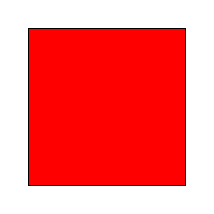
\begin{tikzpicture}
        \draw[fill=red] (0,0) rectangle (2,2) node[pos=0.5]{};
    \end{tikzpicture}
    \caption{rank 0 tensor.}
    \label{fig:r0t}
\end{figure}

\begin{figure}[H]
    \centering 
    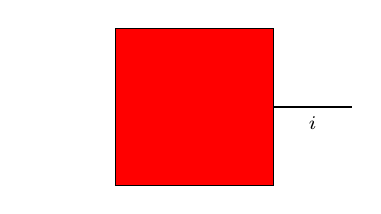
\begin{tikzpicture}
        \draw[fill=red] (0,0) rectangle (2,2) node[pos=0.5]{};
        \draw[](2, 1) -- (3, 1) 
         node[draw=none,fill=none,font=\scriptsize,midway,below]{$i$};
        \draw (-1, 1) node[draw=none]{};
    \end{tikzpicture}
    \caption{rank 1 tensor. Each index is repressented by a line}
    \label{fig:r1t}
\end{figure}

\begin{figure}[H]
    \centering 
    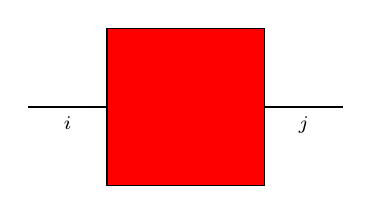
\begin{tikzpicture}
        \draw[fill=red] (0,0) rectangle (2,2) node[pos=0.5]{};
        \draw[](2, 1) -- (3, 1)  
         node[draw=none,fill=none,font=\scriptsize,midway,below]{$j$};
        \draw[](0, 1) -- (-1, 1)  
         node[draw=none,fill=none,font=\scriptsize,midway,below]{$i$};
        
    \end{tikzpicture}
    \caption{rank 2 tensor. Each index is repressented by a line}
    \label{fig:r2t}
\end{figure}

\noindent
Often the indecies are not numbered on these drawing. If we have two tensors we can make them share an index if they have the same dimension, so if we have two rank 3 tensors, one where we have the dimensions of the indexes be 2, 3, 5 and another where it is 1, 4, 3. We can see that they both have an index of size 3 so if we wish we can make them share label for this index. Thus they could have the indecies i, j, k and l, m, j, notice the reuse of j. 

\begin{figure}[H]
    \centering 
    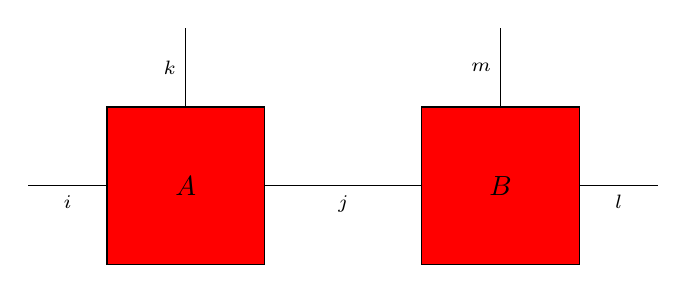
\begin{tikzpicture}
        \draw[fill=red] (0,0) rectangle (2,2) node[pos=0.5]{$A$};
        \draw[](2, 1) -- (3, 1)  
         node[draw=none,fill=none,font=\scriptsize,midway,below]{};
        \draw[](0, 1) -- (-1, 1)  
         node[draw=none,fill=none,font=\scriptsize,midway,below]{$i$};
        \draw[](1, 2) -- (1, 3)  
         node[draw=none,fill=none,font=\scriptsize,midway,left]{$k$};
        
        \draw[fill=red](4,0) rectangle (6,2) node[pos=0.5]{$B$};
        \draw[](6, 1) -- (7, 1)  
         node[draw=none,fill=none,font=\scriptsize,midway,below]{$l$};
        \draw[](4, 1) -- (3, 1)  
         node[draw=none,fill=none,font=\scriptsize,below]{$j$};
        \draw[](5, 2) -- (5, 3)  
         node[draw=none,fill=none,font=\scriptsize,midway,left]{$m$};
    \end{tikzpicture}
    \caption{rank 3 tensors sharing index $j$.}
    \label{fig:2r3t}
\end{figure}

\noindent
But what is this good for? In essence, when we make tensors share indecies it is a way to symbolise that we are multiplying them, matrix multiplication style. The acctual computation of the multiplication can be done at a later point we are just marking our intention. This is important as we might want to build an entire network of tensors and then be strategic about which shared indecies we choose to \textit{contract}. Contracting a shared index is synonumus with computing the product of the two tensors. 
\begin{figure}[H]
    \centering 
    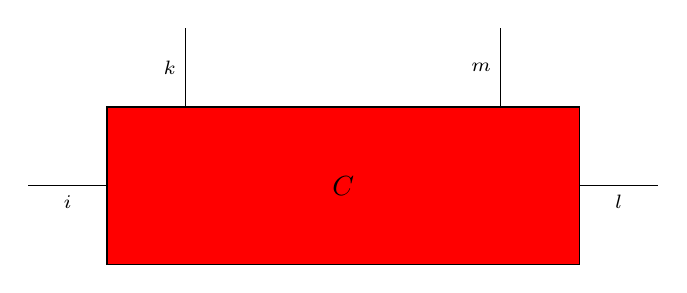
\begin{tikzpicture}
        \draw[fill=red](0,0) rectangle (6,2) node[pos=0.5]{$C$};
        \draw[](0, 1) -- (-1, 1)  
         node[draw=none,fill=none,font=\scriptsize,midway,below]{$i$};
        \draw[](1, 2) -- (1, 3)  
         node[draw=none,fill=none,font=\scriptsize,midway,left]{$k$};
        
        \draw[](6, 1) -- (7, 1)  
         node[draw=none,fill=none,font=\scriptsize,midway,below]{$l$};
        \draw[](5, 2) -- (5, 3)  
         node[draw=none,fill=none,font=\scriptsize,midway,left]{$m$};
    \end{tikzpicture}
    \caption{rank 4 tensor after contracting shared index $j$ from Figure \ref{fig:2r3t}.}
    \label{fig:4t}
\end{figure}
\noindent
in this example we have two tensors A and B where each have elements of the form $a_{ijk}, b_{lmj}$ resulting in a single tensor C with the elements $$c_{iklm}=\displaystyle\sum_{x=0}^{dim(j)-1} a_{ixk}b_{lmx} $$
here $dim(j)=3$ and we subtract 1 since the elements are 0 indexed. In \textit{tensor notation} the summation is implicit if there is a shared index in such an equation so we would just write $c_{iklm}=a_{ijk}b_{lmj}$

\section{Results \& Conclusion}\label{sec:results}
During this project I implemented both the dense and tensor network simulations and here are some results, unless otherwise mentioned all tensor network simulations are run with max bond at 32. 
\begin{figure}[H]
    \begin{center}
        \includegraphics[width=0.45\textwidth]{img/dense_sec_graph.png}
        \includegraphics[width=0.45\textwidth]{img/dense_mem_graph.png}
    \end{center}
    \caption{Time and peak RAM usage from constructing the dense matrices, using the approach discussed in section \ref{sec:dense}.}
    \label{fig:dense_perf}
\end{figure}
\noindent
We see here that both time and memory usage scales faster that quadratic in the number of qubits simulated in the dense simulation. If we look at the tensor network simulation, we see a different picture; time scales quadratically and memory has these spikes but seems to not be affected by the number of qubits after a while. We also notice that before we had to stop at 14 qubits, now we arbitrarily stop at 32 qubits, but if we want, we can run it with 64 qubits in around 30 minutes or larger if we have the time. 
\begin{figure}[H]
    \begin{center}
        \includegraphics[width=0.45\textwidth]{img/tensor_ssec_graph.png}
        \includegraphics[width=0.45\textwidth]{img/tensor_smem_graph.png}
    \end{center}
    \caption{Time and peak RAM usage from constructing the MPOs, using the approach discussed in section \ref{sec:tensor}, compressing after every fifth gate applied.}
    \label{fig:stensor_perf}
\end{figure}
\noindent
The spikes stem from only compressing the MPO every five gates, to confirm this we do the same benchmark where we compress every time. 
\begin{figure}[H]
    \begin{center}
        \includegraphics[width=0.45\textwidth]{img/tensor_sec_graph.png}
        \includegraphics[width=0.45\textwidth]{img/tensor_mem_graph.png}
    \end{center}
    \caption{Time and peak RAM usage from constructing the MPOs, using the approach discussed in section \ref{sec:tensor}, compressing after every gate applied.}
    \label{fig:tensor_perf}
\end{figure}
\noindent
Here we can see the spikes disappear, but we trade it for more time elapsed about 2.5x for 32 qubits. For 64 qubits with a max bond at 65 the difference is 30 minutes against 1 hour and 40 minutes i.e., a 3.3x speedup gained by skipping some compressions. 

\vspace{\baselineskip}
\noindent
Now for the precision, the whole project is built upon the recently proven claim that the singular values are exponentially decreasing in the QFT circuit and therefore we can get most of the precision with a low max bond on the network, here we see a plot of the precision for both the compress every time and every fifth time. 
\begin{figure}[H]
    \begin{center}
        \includegraphics[width=0.45\textwidth]{img/error.png}
        \includegraphics[width=0.45\textwidth]{img/serror.png}
    \end{center}
    \caption{Error obtained by converting the MPO to its dense representation and taking the operator norm of the difference with the exact matrix produced by the dense simulation. Left: compress every time, right: compress every fifth time. }
    \label{fig:tensor_error}
\end{figure}
\noindent
We see here that the error is approximately the same whether we compress every time or every fifth time. We also notice that it decreases less and less and at some point, completely stops improving as we increase the max bond. This is exactly as we expected to see. This is because at some point around a max bond of 40 we keep any relevant data for this circuit even after the compression. If we look at how the memory and time usage is affected by adjusting the max bond, we see that it is a powerful lever for trading precision for performance. 

\begin{figure}[H]
    \begin{center}
        \includegraphics[width=0.45\textwidth]{img/max_bond_sec.png}
        \includegraphics[width=0.45\textwidth]{img/max_bond_mem.png}
    \end{center}
    \caption{Time and peak RAM usage from constructing the MPOs, using the approach discussed in section \ref{sec:tensor}, compressing after every gate applied.}
    \label{fig:tensor_perf_max_bond}
\end{figure}
\begin{figure}[H]
    \begin{center}
        \includegraphics[width=0.45\textwidth]{img/smax_bond_sec.png}
        \includegraphics[width=0.45\textwidth]{img/smax_bond_mem.png}
    \end{center}
    \caption{Time and peak RAM usage from constructing the MPOs, using the approach discussed in section \ref{sec:tensor}, compressing after every fifth gate applied.}
    \label{fig:stensor_perf_max_bond}
\end{figure}
\noindent
The reason we do not extend the graph for the benchmark where we compress every fifth time beyond 47 as max bond is because the spikes in memory usage scale with the max bond and the gap between compressions as seen in the peak memory graph in figure \ref{fig:stensor_perf_max_bond}. 

\vspace{\baselineskip}
\noindent
In conclusion I have implemented enough of the ideas from the paper to see the effects play out and it is indeed far more efficient to simulate the QFT using tensor networks, with close to no error. 

\section{Further work \& acknowledgements}
I unfortunatly did not have time to look into nor implement the zip-up algorithm discussed in the paper which could be someting intersting to work on. 
I would like to acknowledge Michael Kastoryano and Nutan Limaye for their supervision, I would not have been even a third of the way by now without them. I would also like to acknowledge Sebastian Loeschcke for giving a few tips and tricks for working with the python liberary quimb, which saved me many hours.  

\newpage
\nocite{quimb}
\bibliographystyle{plain} % We choose the "plain" reference style
\bibliography{bib}
\newpage
\section{Appendix}
\subsection{Code}
All code used for the project can be found here: \url{https://github.com/AceMouse/quantum-sim} and in the zip file submitted along with this report.
\subsection{calculations for section \ref{sec:maniq}} \label{app:maniq}
\begin{figure}[H]
    \centering
    \begin{align*}
        \qti\ket{\qtz}&=\qi\qz=
        \begin{bmatrix}
            1 \cdot 1 + 0 \cdot 0\\
            0 \cdot 1 + 1 \cdot 0\\
        \end{bmatrix}=
        \qz=\ket{\qtz}\\
        \qti\ket{\qto}&=\qi\qo=
        \begin{bmatrix}
            1 \cdot 0 + 0 \cdot 1\\
            0 \cdot 0 + 1 \cdot 1\\
        \end{bmatrix}=
        \qo=\ket{\qto}
    \end{align*}
    \caption{Applying $\qti$ gate to the states $\ket{\qtz}$ and $\ket{\qto}$}
    \label{fig:app_i}
\end{figure}

\begin{figure}[H]
    \centering
    \begin{align*}
        \qtx\ket{\qtz}&=\qx\qz=
        \begin{bmatrix}
            0 \cdot 1 + 1 \cdot 0\\
            1 \cdot 1 + 0 \cdot 0\\
        \end{bmatrix}=
        \qo=\ket{\qto}\\
        \qtx\ket{\qto}&=\qx\qo=
        \begin{bmatrix}
            0 \cdot 0 + 1 \cdot 1\\
            1 \cdot 0 + 0 \cdot 1\\
        \end{bmatrix}=
        \qz=\ket{\qtz}
    \end{align*}
    \caption{Applying $\qtx$ gate to the states $\ket{\qtz}$ and $\ket{\qto}$}
    \label{fig:app_x}
\end{figure}

\begin{figure}[H]
    \centering
    \begin{align*}
        \qth\ket{\qtz}&=\qh\qz=
        \begin{bmatrix}
            \sqrt{0.5} \cdot 1 + \sqrt{0.5} \cdot 0\\
            \sqrt{0.5} \cdot 1 - \sqrt{0.5} \cdot 0\\
        \end{bmatrix}=
        \qp=\ket{\qtp}\\
        \qth\ket{\qto}&=\qh\qo=
        \begin{bmatrix}
            \sqrt{0.5} \cdot 0 + \sqrt{0.5} \cdot 1\\
            \sqrt{0.5} \cdot 0 - \sqrt{0.5} \cdot 1\\
        \end{bmatrix}=
        \qm=\ket{\qtm}
    \end{align*}
    \caption{Applying $\qth$ gate to the states $\ket{\qtz}$ and $\ket{\qto}$}
    \label{fig:app_h}
\end{figure}

\begin{figure}[H]
    \centering
    \begin{align*}
        \qtr{2}\ket{\qtz}&=\qr{2}\qz=
        \begin{bmatrix}
            1 \cdot 1 + 0 \cdot 0\\
            0 \cdot 1 + \qre{2} \cdot 0\\
        \end{bmatrix}=
        \qz=\ket{\qtz}\\
        \qtr{2}\ket{\qto}&=\qr{2}\qo=
        \begin{bmatrix}
            1 \cdot 0 + 0 \cdot 1\\
            0 \cdot 0 + \qre{2} \cdot 1\\
        \end{bmatrix}=
        \begin{bmatrix}
            0\\
            \qre{2}\\
        \end{bmatrix}=
        \begin{bmatrix}
            0\\
            \mathrm{i}\\
        \end{bmatrix}
    \end{align*}
    \caption{Applying $\qtr{2}$ gate to the states $\ket{\qtz}$ and $\ket{\qto}$}
    \label{fig:app_r2}
\end{figure}

\begin{figure}[H]
    \centering
    \begin{align*}
        \qtcx\ket{\qtz\qtz}&=\qcx
        \begin{bmatrix}
            1\\
            0\\
            0\\
            0\\
        \end{bmatrix}
        =
        \begin{bmatrix}
            1\cdot 1 + 0\cdot 0 + 0\cdot 0 + 0\cdot 0\\
            0\cdot 1 + 1\cdot 0 + 0\cdot 0 + 0\cdot 0\\
            0\cdot 1 + 0\cdot 0 + 0\cdot 0 + 1\cdot 0\\
            0\cdot 1 + 0\cdot 0 + 1\cdot 0 + 0\cdot 0\\
        \end{bmatrix}=
        \begin{bmatrix}
            1\\
            0\\
            0\\
            0\\
        \end{bmatrix}
        =\ket{\qtz\qtz}\\
        \qtcx\ket{\qtz\qto}&=\qcx
        \begin{bmatrix}
            0\\
            1\\
            0\\
            0\\
        \end{bmatrix}
        =
        \begin{bmatrix}
            1\cdot 0 + 0\cdot 1 + 0\cdot 0 + 0\cdot 0\\
            0\cdot 0 + 1\cdot 1 + 0\cdot 0 + 0\cdot 0\\
            0\cdot 0 + 0\cdot 1 + 0\cdot 0 + 1\cdot 0\\
            0\cdot 0 + 0\cdot 1 + 1\cdot 0 + 0\cdot 0\\
        \end{bmatrix}=
        \begin{bmatrix}
            0\\
            1\\
            0\\
            0\\
        \end{bmatrix}
        =\ket{\qtz\qto}\\
        \qtcx\ket{\qto\qtz}&=\qcx
        \begin{bmatrix}
            0\\
            0\\
            1\\
            0\\
        \end{bmatrix}
        =
        \begin{bmatrix}
            1\cdot 0 + 0\cdot 0 + 0\cdot 1 + 0\cdot 0\\
            0\cdot 0 + 1\cdot 0 + 0\cdot 1 + 0\cdot 0\\
            0\cdot 0 + 0\cdot 0 + 0\cdot 1 + 1\cdot 0\\
            0\cdot 0 + 0\cdot 0 + 1\cdot 1 + 0\cdot 0\\
        \end{bmatrix}=
        \begin{bmatrix}
            0\\
            0\\
            0\\
            1\\
        \end{bmatrix}
        =\ket{\qto\qto}\\
        \qtcx\ket{\qto\qto}&=\qcx
        \begin{bmatrix}
            0\\
            0\\
            0\\
            1\\
        \end{bmatrix}
        =
        \begin{bmatrix}
            1\cdot 0 + 0\cdot 0 + 0\cdot 0 + 0\cdot 1\\
            0\cdot 0 + 1\cdot 0 + 0\cdot 0 + 0\cdot 1\\
            0\cdot 0 + 0\cdot 0 + 0\cdot 0 + 1\cdot 1\\
            0\cdot 0 + 0\cdot 0 + 1\cdot 0 + 0\cdot 1\\
        \end{bmatrix}=
        \begin{bmatrix}
            0\\
            0\\
            1\\
            0\\
        \end{bmatrix}
        =\ket{\qto\qtz}
    \end{align*}
    \caption{Applying $\qtcx$ gate to the states $\ket{\qtz\qtz}$, $\ket{\qtz\qto}$, $\ket{\qto\qtz}$ and $\ket{\qto\qto}$}
    \label{fig:app_cx}
\end{figure}

\subsection{calculations for section \ref{sec:maniqi}}\label{app:maniqi}
\begin{figure}[H]
    \centering
    \begin{align*}
        \left(\qti\otimes\qti\otimes\qtx\right)\ket{\qtz\qtz\qtz}=\left(\qi\otimes\qi\otimes\qx\right)\left(\qz\otimes\qz\otimes\qz\right)&= \\
        \begin{bmatrix}
            1
            \begin{bmatrix}
                1 \qx & 0 \qx\\
                0 \qx & 1 \qx\\
            \end{bmatrix}
            & 0
            \begin{bmatrix}
                1 \qx & 0 \qx\\
                0 \qx & 1 \qx\\
            \end{bmatrix}\\
            0 
            \begin{bmatrix}
                1 \qx & 0 \qx\\
                0 \qx & 1 \qx\\
            \end{bmatrix}
            & 1
            \begin{bmatrix}
                1 \qx & 0 \qx\\
                0 \qx & 1 \qx\\
            \end{bmatrix}\\ 
        \end{bmatrix}
        \begin{bmatrix}
            1\\
            0\\
            0\\
            0\\
            0\\
            0\\
            0\\
            0
        \end{bmatrix}
        &=\\
        \begin{bmatrix}
            0 & 1 & 0 & 0 & 0 & 0 & 0 & 0\\
            1 & 0 & 0 & 0 & 0 & 0 & 0 & 0\\
            0 & 0 & 0 & 1 & 0 & 0 & 0 & 0\\
            0 & 0 & 1 & 0 & 0 & 0 & 0 & 0\\
            0 & 0 & 0 & 0 & 0 & 1 & 0 & 0\\
            0 & 0 & 0 & 0 & 1 & 0 & 0 & 0\\
            0 & 0 & 0 & 0 & 0 & 0 & 0 & 1\\
            0 & 0 & 0 & 0 & 0 & 0 & 1 & 0\\
        \end{bmatrix}
        \begin{bmatrix}
            1\\
            0\\
            0\\
            0\\
            0\\
            0\\
            0\\
            0
        \end{bmatrix}
        &=\\
        \begin{bmatrix}
            0\cdot 1 + 1\cdot 0 + 0\cdot 0 + 0\cdot 0 + 0\cdot 0 + 0\cdot 0 + 0\cdot 0 + 0\cdot 0\\
            1\cdot 1 + 0\cdot 0 + 0\cdot 0 + 0\cdot 0 + 0\cdot 0 + 0\cdot 0 + 0\cdot 0 + 0\cdot 0\\
            0\cdot 1 + 0\cdot 0 + 0\cdot 0 + 1\cdot 0 + 0\cdot 0 + 0\cdot 0 + 0\cdot 0 + 0\cdot 0\\
            0\cdot 1 + 0\cdot 0 + 1\cdot 0 + 0\cdot 0 + 0\cdot 0 + 0\cdot 0 + 0\cdot 0 + 0\cdot 0\\
            0\cdot 1 + 0\cdot 0 + 0\cdot 0 + 0\cdot 0 + 0\cdot 0 + 1\cdot 0 + 0\cdot 0 + 0\cdot 0\\
            0\cdot 1 + 0\cdot 0 + 0\cdot 0 + 0\cdot 0 + 1\cdot 0 + 0\cdot 0 + 0\cdot 0 + 0\cdot 0\\
            0\cdot 1 + 0\cdot 0 + 0\cdot 0 + 0\cdot 0 + 0\cdot 0 + 0\cdot 0 + 0\cdot 0 + 1\cdot 0\\
            0\cdot 1 + 0\cdot 0 + 0\cdot 0 + 0\cdot 0 + 0\cdot 0 + 0\cdot 0 + 1\cdot 0 + 0\cdot 0\\
        \end{bmatrix}
        =
        \begin{bmatrix}
            0\\
            1\\
            0\\
            0\\
            0\\
            0\\
            0\\
            0
        \end{bmatrix}
        &=
        \ket{\qtz\qtz\qto}\\
    \end{align*}
    \caption{Applying $\qtx$ to the first qubit in a 3 qubit system}
    \label{fig:app_individual_application1}
\end{figure}


\begin{figure}[H]
    \centering
    \begin{align*}
        \left(\qti\otimes\qtx\otimes\qti\right)\ket{\qtz\qtz\qtz}=\left(\qi\otimes\qx\otimes\qi\right)\left(\qz\otimes\qz\otimes\qz\right)&= \\
        \begin{bmatrix}
            1
            \begin{bmatrix}
                0 \qi & 1 \qi\\
                1 \qi & 0 \qi\\
            \end{bmatrix}
            & 0
            \begin{bmatrix}
                0 \qi & 1 \qi\\
                1 \qi & 0 \qi\\
            \end{bmatrix}\\
            0 
            \begin{bmatrix}
                0 \qi & 1 \qi\\
                1 \qi & 0 \qi\\
            \end{bmatrix}
            & 1
            \begin{bmatrix}
                0 \qi & 1 \qi\\
                1 \qi & 0 \qi\\
            \end{bmatrix}\\ 
        \end{bmatrix}
        \begin{bmatrix}
            1\\
            0\\
            0\\
            0\\
            0\\
            0\\
            0\\
            0
        \end{bmatrix}
        &=\\
        \begin{bmatrix}
            0 & 0 & 1 & 0 & 0 & 0 & 0 & 0\\
            0 & 0 & 0 & 1 & 0 & 0 & 0 & 0\\
            1 & 0 & 0 & 0 & 0 & 0 & 0 & 0\\
            0 & 1 & 0 & 0 & 0 & 0 & 0 & 0\\
            0 & 0 & 0 & 0 & 0 & 0 & 1 & 0\\
            0 & 0 & 0 & 0 & 0 & 0 & 0 & 1\\
            0 & 0 & 0 & 0 & 1 & 0 & 0 & 0\\
            0 & 0 & 0 & 0 & 0 & 1 & 0 & 0\\
        \end{bmatrix}
        \begin{bmatrix}
            1\\
            0\\
            0\\
            0\\
            0\\
            0\\
            0\\
            0
        \end{bmatrix}
        &=\\
        \begin{bmatrix}
            0\cdot 1 + 0\cdot 0 + 1\cdot 0 + 0\cdot 0 + 0\cdot 0 + 0\cdot 0 + 0\cdot 0 + 0\cdot 0\\
            0\cdot 1 + 0\cdot 0 + 0\cdot 0 + 1\cdot 0 + 0\cdot 0 + 0\cdot 0 + 0\cdot 0 + 0\cdot 0\\
            1\cdot 1 + 0\cdot 0 + 0\cdot 0 + 0\cdot 0 + 0\cdot 0 + 0\cdot 0 + 0\cdot 0 + 0\cdot 0\\
            0\cdot 1 + 1\cdot 0 + 0\cdot 0 + 0\cdot 0 + 0\cdot 0 + 0\cdot 0 + 0\cdot 0 + 0\cdot 0\\
            0\cdot 1 + 0\cdot 0 + 0\cdot 0 + 0\cdot 0 + 0\cdot 0 + 0\cdot 0 + 1\cdot 0 + 0\cdot 0\\
            0\cdot 1 + 0\cdot 0 + 0\cdot 0 + 0\cdot 0 + 0\cdot 0 + 0\cdot 0 + 0\cdot 0 + 1\cdot 0\\
            0\cdot 1 + 0\cdot 0 + 0\cdot 0 + 0\cdot 0 + 1\cdot 0 + 0\cdot 0 + 0\cdot 0 + 0\cdot 0\\
            0\cdot 1 + 0\cdot 0 + 0\cdot 0 + 0\cdot 0 + 0\cdot 0 + 1\cdot 0 + 0\cdot 0 + 0\cdot 0\\
        \end{bmatrix}
        =
        \begin{bmatrix}
            0\\
            0\\
            1\\
            0\\
            0\\
            0\\
            0\\
            0
        \end{bmatrix}
        &=
        \ket{\qtz\qto\qtz}\\
    \end{align*}
    \caption{Applying $\qtx$ to the second qubit in a 3 qubit system}
    \label{fig:app_individual_application2}
\end{figure}
\begin{figure}[H]
    \centering
    \begin{align*}
        \left(\qtx\otimes\qti\otimes\qti\right)\ket{\qtz\qtz\qtz}=\left(\qx\otimes\qi\otimes\qi\right)\left(\qz\otimes\qz\otimes\qz\right)&= \\
        \begin{bmatrix}
            0
            \begin{bmatrix}
                1 \qi & 0 \qi\\
                0 \qi & 1 \qi\\
            \end{bmatrix}
            & 1
            \begin{bmatrix}
                1 \qi & 0 \qi\\
                0 \qi & 1 \qi\\
           \end{bmatrix}\\
           1 
           \begin{bmatrix}
               1 \qi & 0 \qi\\
                0 \qi & 1 \qi\\
            \end{bmatrix}
            & 0
            \begin{bmatrix}
                1 \qi & 0 \qi\\
                0 \qi & 1 \qi
            \end{bmatrix}\\ 
        \end{bmatrix}
        \begin{bmatrix}
            1\\
            0\\
            0\\
            0\\
            0\\
            0\\
            0\\
            0
        \end{bmatrix}
        &=\\
        \begin{bmatrix}
            0 & 0 & 0 & 0 & 1 & 0 & 0 & 0\\
            0 & 0 & 0 & 0 & 0 & 1 & 0 & 0\\
            0 & 0 & 0 & 0 & 0 & 0 & 1 & 0\\
            0 & 0 & 0 & 0 & 0 & 0 & 0 & 1\\
            1 & 0 & 0 & 0 & 0 & 0 & 0 & 0\\
            0 & 1 & 0 & 0 & 0 & 0 & 0 & 0\\
            0 & 0 & 1 & 0 & 0 & 0 & 0 & 0\\
            0 & 0 & 0 & 1 & 0 & 0 & 0 & 0\\
        \end{bmatrix}
        \begin{bmatrix}
            1\\
            0\\
            0\\
            0\\
            0\\
            0\\
            0\\
            0
        \end{bmatrix}
        &=\\
        \begin{bmatrix}
            0\cdot 1 + 0\cdot 0 + 0\cdot 0 + 0\cdot 0 + 1\cdot 0 + 0\cdot 0 + 0\cdot 0 + 0\cdot 0\\
            0\cdot 1 + 0\cdot 0 + 0\cdot 0 + 0\cdot 0 + 0\cdot 0 + 1\cdot 0 + 0\cdot 0 + 0\cdot 0\\
            0\cdot 1 + 0\cdot 0 + 0\cdot 0 + 0\cdot 0 + 0\cdot 0 + 0\cdot 0 + 1\cdot 0 + 0\cdot 0\\
            0\cdot 1 + 0\cdot 0 + 0\cdot 0 + 0\cdot 0 + 0\cdot 0 + 0\cdot 0 + 0\cdot 0 + 1\cdot 0\\
            1\cdot 1 + 0\cdot 0 + 0\cdot 0 + 0\cdot 0 + 0\cdot 0 + 0\cdot 0 + 0\cdot 0 + 0\cdot 0\\
            0\cdot 1 + 1\cdot 0 + 0\cdot 0 + 0\cdot 0 + 0\cdot 0 + 0\cdot 0 + 0\cdot 0 + 0\cdot 0\\
            0\cdot 1 + 0\cdot 0 + 1\cdot 0 + 0\cdot 0 + 0\cdot 0 + 0\cdot 0 + 0\cdot 0 + 0\cdot 0\\
            0\cdot 1 + 0\cdot 0 + 0\cdot 0 + 1\cdot 0 + 0\cdot 0 + 0\cdot 0 + 0\cdot 0 + 0\cdot 0\\
        \end{bmatrix}
        =
        \begin{bmatrix}
            0\\
            0\\
            0\\
            0\\
            1\\
            0\\
            0\\
            0
        \end{bmatrix}
        &=
        \ket{\qto\qtz\qtz}
    \end{align*}
    \caption{Applying $\qtx$ to the thrid qubit in a 3 qubit system}
    \label{fig:app_individual_application3}
\end{figure}
\newpage
\noindent
\begin{figure}[H]
    \centering
    \begin{align*}
        \left(\qtx\otimes\qti\otimes\qth\right)\ket{\qtz\qtz\qtz}=\left(\qx\otimes\qi\otimes\qh\right)\left(\qz\otimes\qz\otimes\qz\right)&= \\
        \begin{bmatrix}
            0
            \begin{bmatrix}
                1 \qh & 0 \qh\\
                0 \qh & 1 \qh\\
            \end{bmatrix}
            & 1
            \begin{bmatrix}
                1 \qh & 0 \qh\\
                0 \qh & 1 \qh\\
            \end{bmatrix}\\
            1 
            \begin{bmatrix}
                1 \qh & 0 \qh\\
                0 \qh & 1 \qh\\
            \end{bmatrix}
            & 0
            \begin{bmatrix}
                1 \qh & 0 \qh\\
                0 \qh & 1 \qh\\
            \end{bmatrix}\\ 
        \end{bmatrix}
        \begin{bmatrix}
            1\\
            0\\
            0\\
            0\\
            0\\
            0\\
            0\\
            0
        \end{bmatrix}
        &=\\
        \begin{bmatrix}
        0           &  0          &   0          &   0          &   \sqrt{0.5}      &          \sqrt{0.5} &   0          &   0         \\
        0           &  0          &   0          &   0          &   \sqrt{0.5}      &         -\sqrt{0.5} &   0          &   0         \\
        0           &  0          &   0          &   0          &   0               &          0          &   \sqrt{0.5} &   \sqrt{0.5}\\
        0           &  0          &   0          &   0          &   0               &          0          &   \sqrt{0.5} &  -\sqrt{0.5}\\
        \sqrt{0.5}  &  \sqrt{0.5} &   0          &   0          &   0               &          0          &   0          &   0         \\
        \sqrt{0.5}  & -\sqrt{0.5} &   0          &   0          &   0               &          0          &   0          &   0         \\
        0           &  0          &   \sqrt{0.5} &   \sqrt{0.5} &   0               &          0          &   0          &   0         \\
        0           &  0          &   \sqrt{0.5} &  -\sqrt{0.5} &   0               &          0          &   0          &   0         \\
        \end{bmatrix}
        \begin{bmatrix}
            1\\
            0\\
            0\\
            0\\
            0\\
            0\\
            0\\
            0
        \end{bmatrix}
        &=\\
        \begin{bmatrix}
            0           \cdot 1 +  0          \cdot 0 +   0          \cdot 0 +   0          \cdot 0 +   \sqrt{0.5}      \cdot 0 +          \sqrt{0.5} \cdot 0 +   0          \cdot 0 +   0         \cdot 0\\
            0           \cdot 1 +  0          \cdot 0 +   0          \cdot 0 +   0          \cdot 0 +   \sqrt{0.5}      \cdot 0           -\sqrt{0.5} \cdot 0 +   0          \cdot 0 +   0         \cdot 0\\
            0           \cdot 1 +  0          \cdot 0 +   0          \cdot 0 +   0          \cdot 0 +   0               \cdot 0 +          0          \cdot 0 +   \sqrt{0.5} \cdot 0 +   \sqrt{0.5}\cdot 0\\
            0           \cdot 1 +  0          \cdot 0 +   0          \cdot 0 +   0          \cdot 0 +   0               \cdot 0 +          0          \cdot 0 +   \sqrt{0.5} \cdot 0    -\sqrt{0.5}\cdot 0\\
            \sqrt{0.5}  \cdot 1 +  \sqrt{0.5} \cdot 0 +   0          \cdot 0 +   0          \cdot 0 +   0               \cdot 0 +          0          \cdot 0 +   0          \cdot 0 +   0         \cdot 0\\
            \sqrt{0.5}  \cdot 1   -\sqrt{0.5} \cdot 0 +   0          \cdot 0 +   0          \cdot 0 +   0               \cdot 0 +          0          \cdot 0 +   0          \cdot 0 +   0         \cdot 0\\
            0           \cdot 1 +  0          \cdot 0 +   \sqrt{0.5} \cdot 0 +   \sqrt{0.5} \cdot 0 +   0               \cdot 0 +          0          \cdot 0 +   0          \cdot 0 +   0         \cdot 0\\
            0           \cdot 1 +  0          \cdot 0 +   \sqrt{0.5} \cdot 0    -\sqrt{0.5} \cdot 0 +   0               \cdot 0 +          0          \cdot 0 +   0          \cdot 0 +   0         \cdot 0\\
        \end{bmatrix}
        =
        \begin{bmatrix}
            0\\
            0\\
            0\\
            0\\
            \sqrt{0.5}\\
            \sqrt{0.5}\\
            0\\
            0
        \end{bmatrix}
        &=
        \ket{\qto\qtz\qtp}
    \end{align*}
    \caption{Applying $\qtx$ to the thrid qubit and $\qth$ to the first qubit in a 3 qubit system}
    \label{fig:app_applying_multiple_gates}
\end{figure}

\begin{figure}[H]
    \centering
    \begin{align*}
        \mathbf{U}=\qtcx  \left(\qti\otimes\qth\right) \left(\qti\otimes\qtx\right)&=\\
        \qcx  
        \begin{bmatrix}
            1\qh & 0\qh \\
            0\qh & 1\qh \\
        \end{bmatrix}
        \begin{bmatrix}
            1\qx & 0\qx \\
            0\qx & 1\qx \\
        \end{bmatrix}
        &=\\
        \qcx  
        \begin{bmatrix}
            \sqrt{0.5} &  \sqrt{0.5} & 0 & 0 \\
            \sqrt{0.5} & -\sqrt{0.5} & 0 & 0 \\
            0 & 0 & \sqrt{0.5} &  \sqrt{0.5} \\
            0 & 0 & \sqrt{0.5} & -\sqrt{0.5} \\
        \end{bmatrix}
        \begin{bmatrix}
            0 & 1 & 0 & 0 \\
            1 & 0 & 0 & 0 \\
            0 & 0 & 0 & 1 \\
            0 & 0 & 1 & 0 \\
        \end{bmatrix}
        &=\\
        \begin{bmatrix}
            \sqrt{0.5} &  \sqrt{0.5} & 0 & 0 \\
            \sqrt{0.5} & -\sqrt{0.5} & 0 & 0 \\
            0 & 0 & \sqrt{0.5} & -\sqrt{0.5} \\
            0 & 0 & \sqrt{0.5} &  \sqrt{0.5} \\
        \end{bmatrix}
        \begin{bmatrix}
            0 & 1 & 0 & 0 \\
            1 & 0 & 0 & 0 \\
            0 & 0 & 0 & 1 \\
            0 & 0 & 1 & 0 \\
        \end{bmatrix}
        &=\\
        \begin{bmatrix}
            \sqrt{0.5}  &  \sqrt{0.5} & 0 & 0 \\
            -\sqrt{0.5} &  \sqrt{0.5} & 0 & 0 \\
            0 & 0 & -\sqrt{0.5} & \sqrt{0.5} \\
            0 & 0 & \sqrt{0.5}  & \sqrt{0.5} \\
        \end{bmatrix}& 
    \end{align*}
    \caption{Computing a matrix representation of a circuit,$\mathbf{U}$, that first applies $\qtx$ then $\qth$ to the first qubit then $\qtcx$ to the first and second qubit}
    \label{fig:app_circuit_matrix}
\end{figure}
\begin{figure}[H]
    \begin{alignat*}{2}
        \mathbf{U}\ket{\qtz\qtz}&=
        \begin{bmatrix}
            \sqrt{0.5}  &  \sqrt{0.5}   & 0             & 0          \\
            -\sqrt{0.5} &  \sqrt{0.5}   & 0             & 0          \\
            0           & 0             & -\sqrt{0.5}   & \sqrt{0.5} \\
            0           & 0             & \sqrt{0.5}    & \sqrt{0.5} \\
        \end{bmatrix}
        \begin{bmatrix}
            1 \\
            0 \\
            0 \\
            0 \\
        \end{bmatrix}
        =
        \begin{bmatrix}
            \sqrt{0.5}   \\
            -\sqrt{0.5}  \\
            0            \\
            0            \\
        \end{bmatrix}&=\ket{\qtz\qtm}\\
        \mathbf{U}\ket{\qtz\qto}&=
        \begin{bmatrix}
            \sqrt{0.5}  &  \sqrt{0.5}   & 0             & 0          \\
            -\sqrt{0.5} &  \sqrt{0.5}   & 0             & 0          \\
            0           & 0             & -\sqrt{0.5}   & \sqrt{0.5} \\
            0           & 0             & \sqrt{0.5}    & \sqrt{0.5} \\
        \end{bmatrix}
        \begin{bmatrix}
            0 \\
            1 \\
            0 \\
            0 \\
        \end{bmatrix}
        =
        \begin{bmatrix}
            \sqrt{0.5}   \\
            \sqrt{0.5}   \\
            0            \\
            0            \\
        \end{bmatrix}&=\ket{\qtz\qtp}\\
        \mathbf{U}\ket{\qto\qtz}&=
        \begin{bmatrix}
            \sqrt{0.5}  &  \sqrt{0.5}   & 0             & 0          \\
            -\sqrt{0.5} &  \sqrt{0.5}   & 0             & 0          \\
            0           & 0             & -\sqrt{0.5}   & \sqrt{0.5} \\
            0           & 0             & \sqrt{0.5}    & \sqrt{0.5} \\
        \end{bmatrix}
        \begin{bmatrix}
            0 \\
            0 \\
            1 \\
            0 \\
        \end{bmatrix}
        =
        \begin{bmatrix}
            0            \\
            0            \\
            -\sqrt{0.5}  \\
            \sqrt{0.5}   \\
        \end{bmatrix}&=-\ket{\qto\qtm} \\
        \mathbf{U}\ket{\qto\qto}&=
        \begin{bmatrix}
            \sqrt{0.5}  &  \sqrt{0.5}   & 0             & 0          \\
            -\sqrt{0.5} &  \sqrt{0.5}   & 0             & 0          \\
            0           & 0             & -\sqrt{0.5}   & \sqrt{0.5} \\
            0           & 0             & \sqrt{0.5}    & \sqrt{0.5} \\
        \end{bmatrix}
        \begin{bmatrix}
            0 \\
            0 \\
            0 \\
            1 \\
        \end{bmatrix}
        =
        \begin{bmatrix}
            0             \\
            0             \\
            \sqrt{0.5}    \\
            \sqrt{0.5}    \\
        \end{bmatrix}&=\ket{\qto\qtp}
    \end{alignat*}
    \caption{Applying the circuit represented by the matrix $\mathbf{U}$ from figure \ref{fig:app_circuit_matrix} to different states}
    \label{fig:app_applying_circuit}
\end{figure}

\newpage

\end{document}
% What therory should be better explained?
% make it clear that the singular values exponentially decresing.

% Should i make a pressentation for the exam and how long will the exam be?
% yes, 15 minutes, 10 minutes pressenting what i did, then 5 min live demo in jupyter notebook.

% operator norm of the resulting matricies of 12 qubit version.||M_1 - M_2|| (np.norm(ord=2)) 
